\newcommand{\victor}[1]{{\color{blue}\textbf{[victor:}\textit{#1}\textbf{]}}}
\newcommand{\iris}[1]{{\color{purple}\textbf{[iris:}\textit{#1}\textbf{]}}}
\newcommand{\dimbc}{\mathrm{dim}^{\mathrm{BC}}}
\definecolor{ao(english)}{rgb}{0.0, 0.5, 0.0}
\newcommand{\changed}[1]{{\color{ao(english)}{#1}}}

\section{Introduction}
\label{sec:intro}
\textbf{Hierarchical structures in music}
Music is known to have rich hierarchical structures, ranging from global forms to local phrases, from harmonic progressions to melodic patterns. 
The hierarchical structures allow us to examine music at different levels of details and time scales. 
For example, as shown in Figure \ref{fig:egbach}, the original piece on the top two staffs in can be summarised by the chords in the third staffs; 
similarly, in Figure \ref{fig:egscale}, the patterns shown on the top staff can be progressively and hierarchically reduced to the bottom staff. 
There have been many musical theories on the hierarchical structure of music, such as the General Theory of Tonal Music (GTTM) \cite{lerdahl1985generative} and the Schenkerian theory of melodic reduction \cite{forte1959schenker}.
\begin{figure}[!h]
  \includegraphics[width=\linewidth]{src/img/eg.png}
  \caption{Two levels of hierarchies in Bach's Preludium in C major \cite{wiki:bach}: the original piece and the underlying chords.
          The details in the first two staffs can be summarised into the chords in the third staff}
  \label{fig:egbach}
\end{figure}

\begin{figure}[!h]
  \includegraphics[width=\linewidth]{src/img/egscale.png}
  \caption{Four levels of hierarchies in an artificial example using scales: from the top to the bottom staff, we have different levels of details in different levels of hierarchies.
    The notes at different levels of hierarchies are specified based on the metrical positions of the notes.}
  \label{fig:egscale}
\end{figure}

\textbf{Hierarchies in fractal geometry}
One tool that could be used to study the hierarchical structure in music is fractal theory.
Fractal geometry is an established area of mathematics that studies self-similar patterns on different levels of details.
The concept of fractal dimension has been devised to measure the change of contents across different levels of hierarchies.
\changed{
Because of the imposed recursive rules that generate the hierarchical structures, the fractal dimensions of fractal objects are often not integers; in regular non-fractal objects, however, the dimensions correspond to the common sense definition of dimensions: a square is of fractal dimensions two, and a cube is of fractal dimension three. 
For example, in the one/two-dimensional case of a Koch's snowflake, taking into account of the line segment lengths at different scales (different steps of iterations), it has a fractal dimension $\approx$ 1.26.
Empirically, the fractal dimension can be measured given any contour using the box-counting method, such as the often referenced examples in the geometry of coastlines.
Similarly, given a segment of a melodic line, one can also calculate a parallel of the fractal dimension by looking into the different levels of details exhibited on different levels of hierarchies in the melodic lines.
A detailed mathematical description is given in \secref{sec:fractal-geom}.}

\textbf{Related Work}
In the research area of MIR, many useful tools and investigation have been made to understand the hierachical structures of music.
For example, there are music musical analysis assistant \cite{hamanaka2009interactive, hamanaka2005atta}, compositional tools \cite{hamanaka2004automatic, hamanaka2005automatic}, evaluation investigation \cite{mcfee2017evaluating, mcfee2015hierarchical} based on a variety of hierachical structure analysis in music.
Self-similarity concepts, and fractals in particular have inspired many research in audio and music analysis \cite{bigerelle2000fractal,hsu1990fractal,hsu1991self} and composition \cite{sukumaran2009generation,leach1995nature}.
In other domain of applications, the fractal theory has been widely used in investigating time series, dynamical systems, and non-linearity \cite{accardo1997use, higuchi1988approach}.
To the best of our knowledge, there has not been an attempt on computing the fractal dimensions equivalent in symbolic music by drawing the parallel between the box-counting method and hierarchical structures in music. 

\textbf{Musical patterns}
Using the fractal dimensions, we showcase its effectiveness by applying it to
musical pattern discovery. 
Musical patterns are easily spotted by a trained performer,
even if the pattern appears under different \emph{variations}.  These
variations include transpositions, inversions, time dilations (\iris{augmentation, diminuation}), between
others. Amongst the favorite examples of patterns showing up under a
plethora of variations are the fugues by J.S. Bach. Take
\Cref{fig:bwv861-start}, we see two patterns showing up under
inversions and transpositions in the first two bars.

\begin{figure}
  
\includegraphics[width=\linewidth]{src/img/bwv861-start-section-patterns.pdf}
  \caption{Two patterns and their variations in the beginning of BWV 861}
  \label{fig:bwv861-start}
\end{figure}

Writing a computer program that is capable to identify these patterns modulo their variations is no easy feat.
\changed{The challenges in musical pattern discovery has been detailed in \cite{janssen2013finding, meredith2015music,ren153analysis}. }
The naive approach
would be to select a candidate pattern, then go over the whole
piece comparing interval per interval. This would have to be computed
for every possible pattern candidate. The exponential nature of this
approach makes it unrealistic and will not get us very far.

  In this paper we discuss an alternative, and efficient, approach to
identifying patterns in symbolic music. The idea is to assign a real
number to a potential pattern in such a way that \emph{similar}
patterns have \emph{similar} numbers. We call this the pattern
identifier.  This enables us to group patterns that differ by
$\epsilon$.  A potential pattern consists simply in a group of
notes. If we want to check whether a pattern of $n$ notes shows up but
in half tempo, for example, we can compute the pattern identifier for
all groups of contiguous $2n$ notes and compare the pattern
identifiers.  

  Defining the pattern identifier as the Minkowski-Bouligand
dimension~\cite{bouligand1928ensembles} is a prime option in our
arsenal.  This is also known as the Box-Count (BC) dimension, and we
shall denote it by $\dimbc$. There are two main reasons for choosing
the Box-Count dimension for our identifier: (A) it is simple to
approximate by computational means, and, (B) it approximates the
fractal dimension of a shape.  These reasons make a good case
together. We must be able to efficiently compute the pattern
identifier and it must identify similar patterns with at most
$\epsilon$ distance, where similar here means inversions,
transpositions and time-dilations. Fractals are self-similar to
rotated, translated or scaled out versions of themselves, and hence
share a common dimension. Consequently, beind able to efficiently
compute an approximation for this dimension is key.  


\victor{ It is worth
noting that usinc fractal dimensions might give false positives, for
we need to perform some check after correlating the fractal dimensions
of different candidates. Nevertheless, this process allows us to focus
our computational resources and analyze only candidate occurences of
patterns that are likely to be, in fact, the same pattern. }

\iris{The fractal dimension also *guarantee* to give us back the patterns that went through rigid/symmetric (e.g. inversion, retrograde, inversion-retrograde) transformations. 
So if people are not looking for retrograde, then there is a *guaranteed* false positive of retrograde. 
We can prove this mathematically. 
Could be a paragraph in the next seciton? 
Just to clarify that we can also be more precise and certain on what kind of patterns are extracted. } 




  Our contributions are summarized below.

\begin{itemize}
  \item We provide a novel adaptation of fractal geometry for identifying patterns
        in a musical piece under a number of variations.
  \item We have implemented our analisys as a library and made it publicly available.
  \item We have empirically shown the effectiveness of our method for musical pattern
        recognition by running our tool in a number of musical pieces.
\end{itemize}

\section{The Fractal Geometry of Symbolic Music}
\label{sec:fractal-geom}

  % In this section we review the necessary parts of fractal geometry
% and explain how to apply it to symbolic music notation. This enables
% us to identify a pattern with a number that is constant under
% variations such as transpositions, inversions, time dilations, etc.

\changed{
Mathematically, the fractal dimension is defined as $$D=-\frac{logM}{logs}$$
where $M=Mass$, usually defined in terms of lengths or areas of the geometric objects, and $s=scaling$, usually defined as how many recursive steps has been taken in creating the fractals.

One intuition of fractal dimension is how rough or how much detail are embedded in the geometric object.
Continuing on the example from the introduction section, the coastlines of different countries can be measured in terms of fractal dimensions by using the box-counting method \cite{sarkar1994efficient}, where one control the scaling factor $s$ and count the ``boxes'' to obtain the mass $M$.
Thus we can empirically compute fractal dimensions given any geometric objects. 
}

 In more detail, the box-count (BC) dimension~\cite{bouligand1928ensembles} of a shape
can be seen as a measure of the \emph{roughness} of that shape. It coincides with the
Euclidean dimension for the familiar shapes but it might be non integer. For example,
the BC-dimension of the Sierpinski Triangle (\Cref{fig:egboxcount}, right) is $\log_2 3 \approx 1.585$

  We can calculate the box-count (BC) dimension of a shape through a
process known as box-counting. The idea is simple. We lay a shape in a
grid and count how many squares it touches, call it $N$, then scale
the shape by a factor $s$ and count how many quares it touches again,
call it $N_s$. The box-counting dimension $d$ of the given shape is
defined by the value that $\log_s(\frac{N_s}{N})$ converges to, for
growing values of $s$.  Since this limit might not exist, it is common
to consider the upper and lower box-count dimensions.  For our
purposes, we can safely ignore these complications. In fact, we will
only approximate the BC-dimension of a shape by considering a discrete
number of scalings. \victor{why can we do this? Well, Since false positives exist anyway,
  why care so much for extreeme precision?}

\begin{figure}
  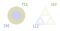
\includegraphics[width=\linewidth]{src/img/box-counting-example-alt.pdf}
  \caption{Box counting applied to a circle and the Sierpinsky Triangle. The numbers
indicate the number of boxes touched by the object before and after scaling by a factor of 2.}
  \label{fig:egboxcount}
\end{figure}


In \Cref{fig:egboxcount} we show box-counting being applied to a
circle and the Sierpinski Triangle. On the left we see a small circle,
touching 186 boxes, and a circle double the size of the first,
touching 714.  The circle has a known dimension of 2. On the right we
see the same for the Sierpinski Triangle, which has a known fractal
dimension of $\log_2 3 \approx 1.585$.  If we apply the BC dimension
formula to the data in \Cref{fig:egboxcount} we obtain:

\[
\begin{array}{l l l l}
  \dimbc (\mathrm{circle}) &= \log_2{\frac{714}{186}} &= 1.94 &\approx 2 \\[.5em]
  \dimbc (\mathrm{sierp})  &= \log_2{\frac{363}{122}} &= 1.57 &\approx 1.585 \\
\end{array}
\]

  We see that the dimension our data gives is just
\emph{approximately} the correct value, but it serves its purpose
perfectly for our objective: to isolate pattern candidates that have
no connection whatsoever. Note that this number distinguishes the
the circle from the Sierpinski Triangle for any $\epsilon < 0.37$,
which is a \emph{big} margin. Moreover, if we rotate, translate 
to another position in the plane, or even scale the circle and
Sierpinski triangle, their approximated BC dimension stays the same.

%% If we were to iterate this
%% process and plot the number of boxes touched by the scaled version of
%% our shapes, over the scale factor, we would see that the data for the
%% circle fits almost perfectly fit the curve $f(x) = cx^2$, for $c$
%% being a constant. The Sierpinski triangle would fit the curve $f(x) =
%% cx^{1.585}$.  That is, for a given shape with BC dimension $d$, the
%% number of boxes touched by the shape scaled by $s$ gets closer and
%% closer to $cs^d$ as $s$ grows.

  We have seen how the approximate BC-dimension of a shape is a good
measure for isolating occurences of a pattern minus false positives.
In order to apply this to symbolic music, however, we must define what
do we mean by \emph{scaling} in symbolic music.

\subsection{Scaling and BC-dimension in Music}
In the context of music, there have been evidences that a visual-audio correspondence exists amongst music objects \cite{thorpe2016perception}.
This can also be observed from the sheet music.
Without musical training, one can differentiate the uneven, irregular contours of music notes against the smooth, regular contours, and have certain expectations in the corresponding musical events.
Following the intuition given in the last paragraph, a rougher contour which contains many details would correspond to a higher ``Mass'' in terms of the fractal geometry.
Different measures can be defined to measure the mass of melodic contour.
In this paper, we take a simple mass measurement
$$M(n_1, n_2) = \sqrt{(t_1-t_2)^2 +(p_1-p_2)^2}$$
  where $n_i=(t_i, p_i)$, that is, a musical note is characterised by its onset time and the pitch number. 
Intuitively, it is the line segment between two notes.
By taking the sum of the line segments, we obtain the length sum approximating the roughness of the contour of a melodic line.

Note values provide a simple notion of scaling, or considerations at different
granularity in time, for symbolic music.
Take a piece of music and look only on one note every time a metronome
beats on a quarter note. Now do the same but change the metronome to
click on every sixteenth note. The second pass will uncover, in general,
more detail than the first. This is a crucial observation. The notion
of scaling, specially in the fractal geometric sense, is tightly tied
to the notion of detail. The closer we look at a shape, the more detail we see.
This process put the music surface to a hierarchy of melodic reduction: the
courser the time granularity, the more reduced the details in the melody would be. 
Given such a hierarchy of melodic reduction, we can ``zoom-in/out'' across the hierarchy and examine have different levels of details.

  In \Cref{fig:egscalingmusic} we show an example of looking at the first
measure in J. S. Bach's first Cello Suite on different scales. We start at 
a more coarse scale, the half note, and progress to a finer scale, the sixteenth note.
We also connect the notes we see on each respective scaling factor.

\begin{figure}
  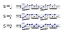
\includegraphics[width=\linewidth]{src/img/musical-scaling-example.pdf}
  \caption{The ``box-count'' under different scalings for the first measure in BWV 1007,
the numbers indicate the length, in pixels, for their respective lines.}
  \label{fig:egscalingmusic}
\end{figure}

  \victor{There are a number of notions one could consider, for example
blah, inner metric (cite Anja's inner metric), blih or bloh. We leave
those for future work and use a simpler version}

  Next, in order to approximate the BC-dimension of a group of notes
we can apply the same process as in \Cref{fig:egboxcount}. Counting boxes for
a figure in the plane is a way of approximating the area, also called
the \emph{mass} of the shape. For a line it is quite easy to calculate
the mass directly: it is the length of that line. Hence, if we take 
the lines in \Cref{fig:egscalingmusic}, they measure $308$ at scale
$s$, $390$ at scale $2s$ and $485$ at scale $4s$. With this data
at hand, we can approximate the BC-dimension of the first measure in
BWV 1007:

\[
\begin{array}{l l l}
 \dimbc (\mathrm{BWV1007}_1)  &\approx \log_2 \frac{390}{308} &= 0.340 \\[.5em]
                              &\approx \log_4 \frac{485}{308} &= 0.327 \\
\end{array}
\]

\victor{finish this}

\iris{The explanation computation on Figure \ref{fig:egscalingmusic} is very clear, 
but should we still describe how we calculated the mass in the actual midi number and duration? 
We are not taking the pixels after all? It might confuse people in optical score recognition research?  }

% \textbf{A simplified example to compute the features}
% First, we split a music entry into m parts, n bars per part.
% We then perform the following actions for each bar: take the notes in the most
% important positions in the bar.
% For example, in a 4/4 bar, we have a importance grid of [5,2,3,2,4,2,3,2] in the resolution of a quiver. 
% Only the notes on position of the first quiver will be taken. 
% Take the notes in the most and the second most important positions in the bar 
% (we have the positions of the first and the fifth quiver in this case); 
% repeat till we consider all the importance level. 
% Next, we compute measurement (mass) on the hierarchy. 
% Calculate the mass within one note: = duration in quarter length; 
% Calculate the mass between two notes =  $\sum \sqrt{\Delta duration^2 + \Delta pitch^2}$ (eqv to the hypotenuse of the time and frequency difference). 
% Finally, we sum up the mass (intuitively as the length of the line tracing through the notes in considerations. 
% The last step is to take ratios and the log of the mass between the selected two
% hierachies: $dim = log_2(mass_{I1}/mass_{I2})$.


% \textbf{Similarity dimension in music}
% And given a hierarchy of melodic reduction, we can ``zoom-in/out'' across the hierarchy and examine have different levels of details, which can function as the scaling $s$.
% Therefore, in a monophonic scenario, we can calculate a similarity dimension using two levels in musical hierarchy using $M$ and $s$. 

\changed{

\subsection{Parameters}
From the descriptions above, we need to decide at least the scope and the zooming levels for calculating the fractal dimensions:
\begin{itemize}
\item Window size (g): integers indicating how many bars are used for the computation at a time. 
\item Zoom levels (z): two integers indicating which levels on the hierarchy we are computing the fractal dimensions with. 
\end{itemize}

There is also an option to use a hopping or a sliding window. 
Our default set of parameters are $g=2$, $z=(2,1)$ with hopping window. 

\subsection{Properties of Fractal Dimension}
From the computation defined in the last subsection, we are guaranteed to extract certain types of patterns.
We give mathematical accounts for such connections in this section.

% \textbf{Mirror forms}
\textbf{Symmetric musical transformation}
There are certain circumstances where the following rigid symmetric musical transformations do not change the fractal dimensions.

\begin{itemize}
\item Inversion: reverse pitch intervals
\item Retrograde: mirror pitches and durations backwords
\item Inversion-Retrograde: the composition of inversion and then retrograde
\item Retrograde-Inversion: the composition of retrograde and then inversion
\end{itemize}

We can show that the inversion transformation do not affect the fractal dimension, however, this is not the case for other transformations on the list.

For proving that the fractal dimension is an invariance under the inversion transformation, we only need to show that the mass of the melodic line do not change after the transformations. 
We use $M$ for taking the mass, $D = [(t_1, p_1), (t_2,p_2),...]$ stands for the input music data in the form of time-pitch pairs, and $I, R, IR, RI$ stands for the transformations.

By definition of the mass calculation, we have:
$M(D) = \sum\limits_n ((t_n-t_{(n+1)})^2 + (p_n - p_{n+1})^2)^{\frac{1}{2}} $
For inversion, we have $M(I(D))$:
\begin{flalign*}
  \tiny
&= M(I([(t_1, p_1), (t_2,p_2),...]))&\\
&= M([(t_1, p_1), (t_2, p_1-(p_2-p_1),&\\
& \qquad (t_3, p_1 - (p_2-p_1) - (p_3-p_2), ...))])&\\
&= ((t_1-t_2)^2 + (p_2 - p_1)^2)^{\frac{1}{2}}&\\
& \qquad + ((t_2-t_3)^2 + (p_2 - p_3)^2)^{\frac{1}{2}} + ...&\\
&= M(D)
\end{flalign*}

For retrograde, in general,
\[
 \sum\limits_n(\Delta t_n + \Delta p_n)^{\frac{1}{2}} - \sum_{\substack{n=1,2,...,T \\ m=T,T-1,...,1}}(\Delta t_{m} + \Delta p_n)^{\frac{1}{2}} \neq 0
\]

unless $\Delta t_n = \Delta t_m$, that is, when the time intervals exhibit a symmetry with respect to the middle time interval.
However, since the difference (the left hand side of the equation) is a polynomial function, we can expect that the fractal dimension does not change drastically after the retrograde transformation. 

\textbf{Ornamentation and simplification}
When we add in a note or subtract a note, as long as the changed notes do not enter the set of important notes we consider, the fractal dimensions remain the same.
}

\section{Experiment}

\victor{Describe the setup: wrote some haskell code,
got some data from MIDI, mined for patterns using technique shown in \Cref{sec:fractal-geom}}


\textbf{Simple Examples}
As an example, we plot the similarity dimension time series in Hanon, as shown in \figref{fig:simpeg}.
The symmetric structure of the piece was captured by the time series of fractal dimensions.

\begin{figure}
  \includegraphics[width=\linewidth]{src/img/frac-simpeg.pdf}
  \caption{The fractal dimensions of patterns in the Hanon Exercise No.6. Each data point corresponds to the four-bar window we took.  }
  \label{fig:simpeg}
\end{figure}

\textbf{Correlation with existing features}
By comparing with other musically meaningful features, we verify that the BC-dimension is not redundant. 
At p-value threshold 0.01, the fractal feature only correlates with three features out of the 150 features in jSymbolic2.2, Mean Pitch, Pitch Skewness, Variability of Partial Rest Durations. 

\textbf{Distance matrix}
By taking different distance measures, we can use the devised fractal dimensions for classification purposes.
\begin{figure}
  \includegraphics[width=\linewidth]{src/img/fragemdist.pdf}
  \caption{The distance matrix of the fractal dimension time series. }
  \label{fig:simpeg}
\end{figure}

\changed{
\textbf{Pattern discovery}
We can extract patterns based on the fractal dimensions as shown in \figref{fig:extract}.
This monophonic version of the Mozart piece is one out of five pieces in the JKU-PDD dataset.
Due to space limit, we only show one pattern that is extracted by the tool with our default setting.
An exploration using a full parameter sweep is out of scope of this paper.
The pattern discovery functionality is packaged with our analysis tool, which can be accessed online.\footnote{\url{https://github.com/xxx/hs-fragem}}.
As expected, the exact repetitions are all foregrounded in the newly generated MIDI file.
For a long MIDI file with low readability, our tool could be useful for highlighting the repetitions across the piece.

Although we do not conduct a comprehensive comparison to other existing musical pattern discovery algorithms~\cite{meredith2016using,velarde2016wavelet,pesek2017symchm,collins2013siarct,conklin2002representation,conklin2010discovery,ren2016closed}, our methods feature an end-to-end compiled application for pattern discovery in music. 
There is also a recent web-based tool that find patterns with a certain degree of flexibility in jazz solos~\cite{FrielerHPD18}; our tool has more considerations with the hierarchical structures in music. 
}

\begin{figure*}
  \includegraphics[width=\linewidth]{src/img/fragempat.pdf}
  \caption{Using fractal dimensions to extract repeated patterns in a monophonic version of Mozart's Piano Sonata No.4 in E-flat major, K282, second movement. Our tool extract patterns from a MIDI file and generate a new MIDI file with the presence of the patterns only. }
  \label{fig:extract}
\end{figure*}


\section{Discussion and Conclusion}
 
\victor{we need a better phrase or two about related
work, in the lines of: Although Fractal Geometry and Music goes a long way\cite{bigerelle2000fractal,hsu1990fractal,hsu1991self},
we are applying it to a novel part in music analisys.}

\iris{Newly added: }

\textbf{Future Work}
Polyphony would be a ntural extension for the work. 
For multiple voice, one can extend the dimension and devise a new measure for mass. 
It would be interesting to see how the fractal dimensions correspond to previously defined harmonic similarity measures. 

\textbf{Conclusion}
Based on the parallels between the hierarchical structures in music and fractals, we used the box-counting method to compute the fractal dimensions in monophonic symbolic music.
The fractal dimension has a low correlation to existing features of symbolic music, and therefore contributes to new perspective on a combined view of pitch and rhythm.
We provide a tool for pattern discovery based on this feature. 

%% 
%% It is worth noting that this
%% values converges very slowly.  \victor{I'm not very attached to the plot \Cref{fig:egplots},
%% maybe use it just in case we need to fill in space?} In \Cref{fig:egplots} we see the data we
%% gathered through box counting both the circle and the Sierpinski
%% triangle plotted against the curve of their known BC dimension.
%% 
%% 
%% \begin{figure}
%% \begin{tikzpicture}
%% \begin{axis}[
%%   legend pos=north west
%% ]
%% \addplot [mark=*,blue,only marks,opacity=0.5] table {
%% 0  0
%% 1  186
%% 2  714
%% };
%% \addlegendentry{box-count Circle}
%% \addplot [mark=*,red,only marks,opacity=0.5] table {
%% 0 0
%% 1 122
%% 2 363
%% };
%% \addlegendentry{box-count Sierp.}
%% \addplot [no marks,color=black!40!blue,domain=0:3] expression {
%%   (814 / 4) * x ^ 2
%% };
%% \addlegendentry{$f(x) = c\times x^{2\textcolor{white}{.0000}}$}
%% \addplot [no marks,color=black!40!red,domain=0:3] expression {
%%   (412 / 2^1.5) * x ^ 1.5849
%% };
%% \addlegendentry{$f(x) = c\times x^{1.5849}$}
%% \end{axis}
%% \end{tikzpicture}
%% \caption{Plot of the data obtained through box counting (\Cref{fig:egboxcount})
%% versus the known dimensions of the objects.}
%% \label{fig:egplots}
%% \end{figure}

% two figures from the first version
